% Autor: Leonhard Segger, Alexander Neuwirth
% Datum: 2017-10-30
\documentclass[
	% Papierformat
	a4paper,
	% Schriftgröße (beliebige Größen mit „fontsize=Xpt“)
	12pt,
	% Schreibt die Papiergröße korrekt ins Ausgabedokument
	pagesize,
	% Sprache für z.B. Babel
	ngerman
]{scrartcl}

% Achtung: Die Reihenfolge der Pakete kann (leider) wichtig sein!
% Insbesondere sollten (so wie hier) babel, fontenc und inputenc (in dieser
% Reihenfolge) als Erstes und hyperref und cleveref (Reihenfolge auch hier
% beachten) als Letztes geladen werden!

\usepackage{tikz}
\usetikzlibrary{calc,patterns,angles,quotes} % loads some tikz extensions\usepackage{tikz}
\usetikzlibrary{babel}

% Silbentrennung etc.; Sprache wird durch Option bei \documentclass festgelegt
\usepackage{babel}
% Verwendung der Zeichentabelle T1 (Sonderzeichen etc.)
\usepackage[T1]{fontenc}
% Legt die Zeichenkodierung der Eingabedatei fest, z.B. UTF-8
\usepackage[utf8]{inputenc}
% Schriftart
\usepackage{lmodern}
% Zusätzliche Sonderzeichen
\usepackage{textcomp}

% Mathepaket (intlimits: Grenzen über/unter Integralzeichen)
\usepackage[intlimits]{amsmath}
% Ermöglicht die Nutzung von \SI{Zahl}{Einheit} u.a.
\usepackage{siunitx}
% Zum flexiblen Einbinden von Grafiken (\includegraphics)
\usepackage{graphicx}
% Abbildungen im Fließtext
\usepackage{wrapfig}
% Abbildungen nebeneinander (subfigure, subtable)
\usepackage{subcaption}
% Funktionen für Anführungszeichen
\usepackage{csquotes}
\MakeOuterQuote{"}
% Zitieren, Bibliografie
\usepackage[sorting=none]{biblatex}


% Zur Darstellung von Webadressen
\usepackage{url}
%chemische Formeln
\usepackage[version=4]{mhchem}
% siunitx: Deutsche Ausgabe, Messfehler getrennt mit ± ausgeben
\usepackage{floatrow}
\floatsetup[table]{capposition=top}
\usepackage{float}
% Verlinkt Textstellen im PDF-Dokument
\usepackage[unicode]{hyperref}
% "Schlaue" Referenzen (nach hyperref laden!)
\usepackage{cleveref}
\sisetup{
	locale=DE,
	separate-uncertainty
}
%\bibliography{Raster-Kraft-Mikroskopie_References}

\begin{document}

	\begin{titlepage}
		\centering
		{\scshape\LARGE Versuchsbericht zu \par}
		\vspace{1cm}
		{\scshape\huge AFM - Raster-Kraft-Mikroskopie \par}
		\vspace{2.5cm}
		{\LARGE Gruppe BA-C-04 \par}
		\vspace{0.5cm}

		{\large Alexander Neuwirth (E-Mail: a\_neuw01@wwu.de) \par}
		{\large Leonhard Segger (E-Mail: l\_segg03@uni-muenster.de) \par}
		\vfill

		durchgeführt am 05.11.18\par
		betreut von\par
		{\large Anne Bakker}

		\vfill

		{\large \today\par}
	\end{titlepage}
	\tableofcontents
	\newpage

	%TODO mehr TODO in Default

	\section{Kurzfassung}
	%TODO Hypothese	und deren Ergebnis, wenn Hypothese ist, dass nur Theorie erfüllt, sagen: Erwartung: Theorie aus einführung (mit reflink) erfüllt
	%TODO Ergebnisse, auch Zahlen, mindestens wenn's halbwegs Sinn ergibt
	%TODO Was wurde gemacht
	%TODO manche leute wollen Passiv oder "man", manche nicht

	\section{Theorie}

	\section{Methoden}
	%TODO Bilder von der Website klauen
	%TODO einer will Präsens

	\section{Ergebnisse und Diskussion}
	%TODO Unsicherheiten


	\subsection{Beobachtung}
	%TODO Einflüsse von veränderten Parametern auf Messung
	\subsubsection{Unsicherheiten} %TODO GGF IN DATENANYLSY
	Folgende Unsichheiten waren auf den Behältern der Cantilevers für die Federkonstante $c$ angegeben:
	\begin{description}
		\item[statischer Modus:] \SI{0.02}{N/m} - \SI{0.77}{N/m}
		\item[dynamischer Modus:] \SI{21}{N/m} - \SI{98}{N/m}
	\end{description}
	Alle weiteren Unsicherheiten verschwinden gegenüber der Unsichheit der Federkonstante.
	\subsection{Datenanalyse}
	%TODO Berechung nach Aufgabenstellung
	\subsubsection{Kalibrierungsprobe}
	Die Adhäsionskräft, welche an einem Punkt auf den Cantilever wirkt, während dieser sich von dem Material wegbewegt, lässt sich direkt aus dem Snap-off s und der Federkonstante bestimmen:
	\begin{equation}
			F_\text{adh} = \Delta s \cdot c
	\end{equation}
	Es folgt $F_\text{adh}=\SI{10.8+-11.4}{nN}$, wobei über die fünf gemessenen Hysteresen (\crefrange{fig_kali_ds1}{fig_kali_ds5}) gemittelt wird.
	\subsubsection{CD/DVD/BR}
	\subsubsection*{DVD}
	% 1) DVD
	% 2) CD
	% 3) BR
	\subsubsection{Spitzenradius} %TODO Name
		\subsection{Diskussion}
	%TODO Bezug/Nutzen oder sonst was
	%TODO auch hier die Hypothese wiederholen
	%TODO keine Messwerte hier, nach manchen Menschen, zumindest "direkt" erstellte Diagramme net hier, auch wenn Lesbarkeit-bla

 %TODO vegleich literatur Box+ Nanosurf spitzen radius
\begin{table}[H]
	%TODO tabelle für zusammen vergleichen der Adhäsionskräfte?
		\centering
		\begin{tabular}{ c | c }
			 & Kalibrierungsprobe\\ \hline
			$F_\text{adh}$ & \SI{10.8+-11.4}{nN} \\ %26.287, 28, 25.557, 35.1, 29.6
		\end{tabular}
		\caption{Adhäsionskräfte die auf die Spitze des Cantilevers wirken bei Kraft-Abstand-Spektroskopie.} %TODO mehr
		\label{tb_ds}
	\end{table}

	%TODO CD/DVD https://www.nickles.de/c/s/Klein-rund-und-duenn-was-steckt-in-der-DVD-267-1.html sonst findet man auch mit spurbreite googlei für BR

	\section{Schlussfolgerung}
	%TODO Rückgriff auf Hypothese und drittes Nennen dieser

	%TODO Quellen zitieren, Websiten mit Zugriffsdatum
	%TODO Verweise auf das Laborbuch (sind erlaubt)
	%TODO Tabelle + Bilder mit Beschriftung
	%\printbibliography
	\section{Anhang}

\begin{figure}[H]
			\subcaptionbox{Draufsicht \label{fig_kali_top}}{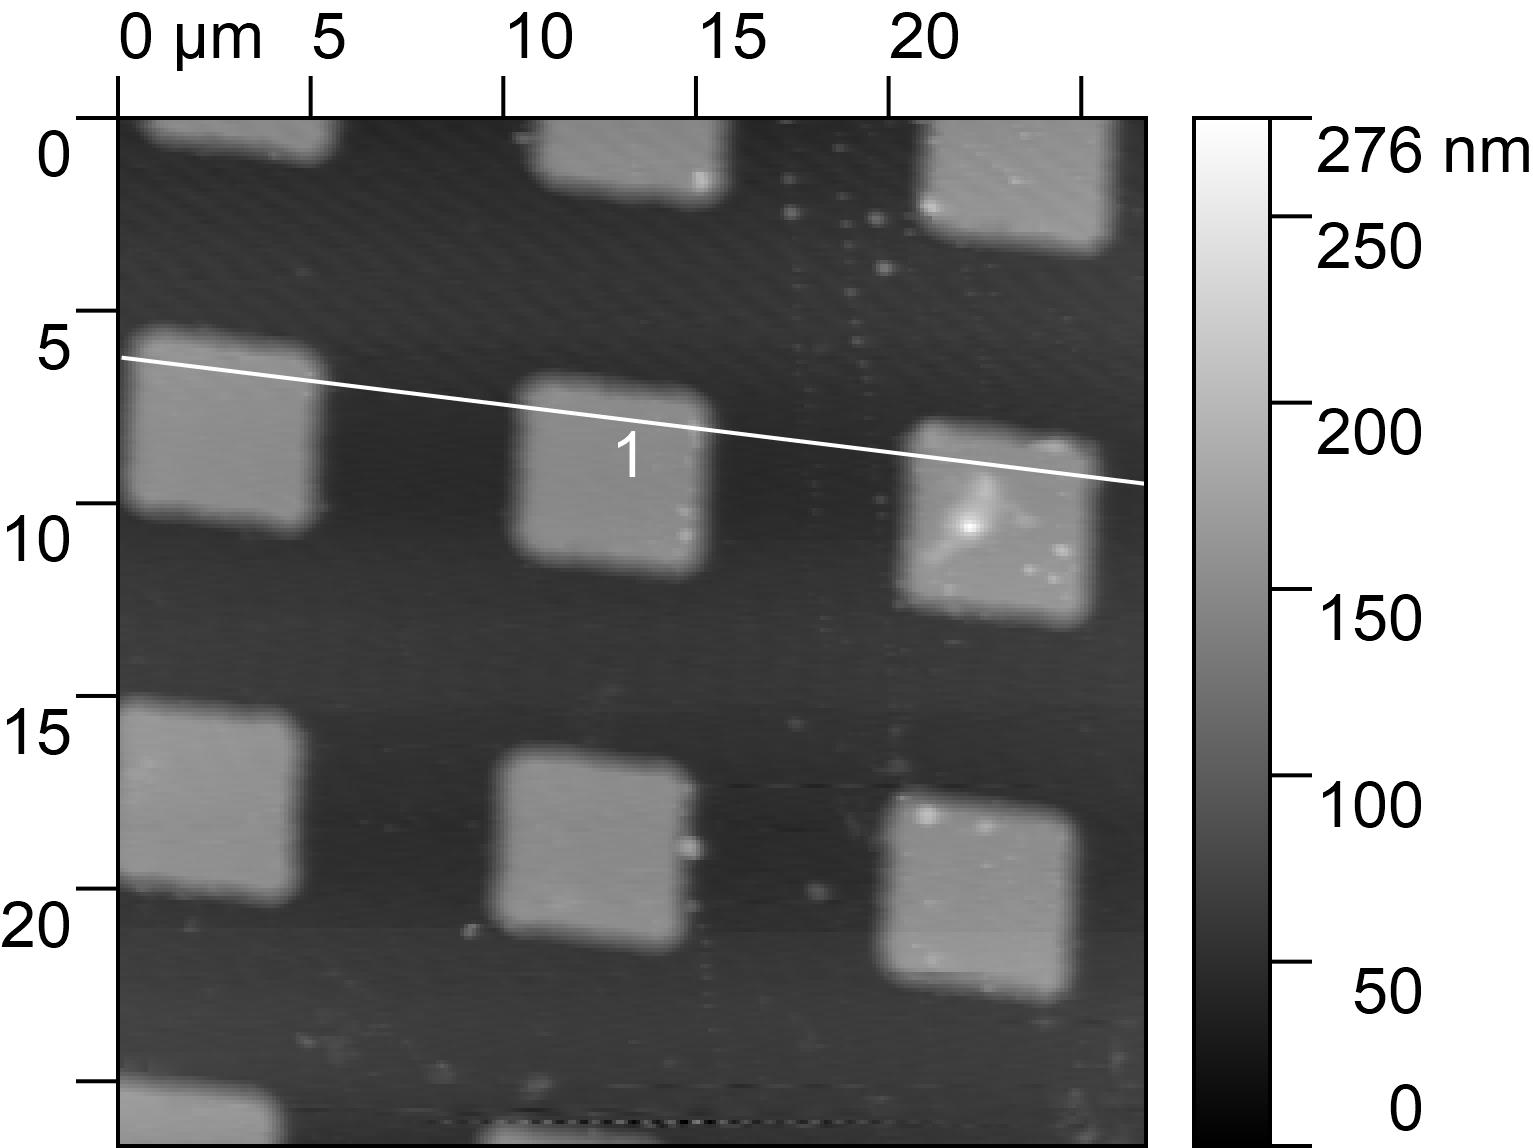
\includegraphics[width=.49\linewidth]{images/Kali/Top}}
			\subcaptionbox{3D-Sicht \label{fig_kali_3d}}{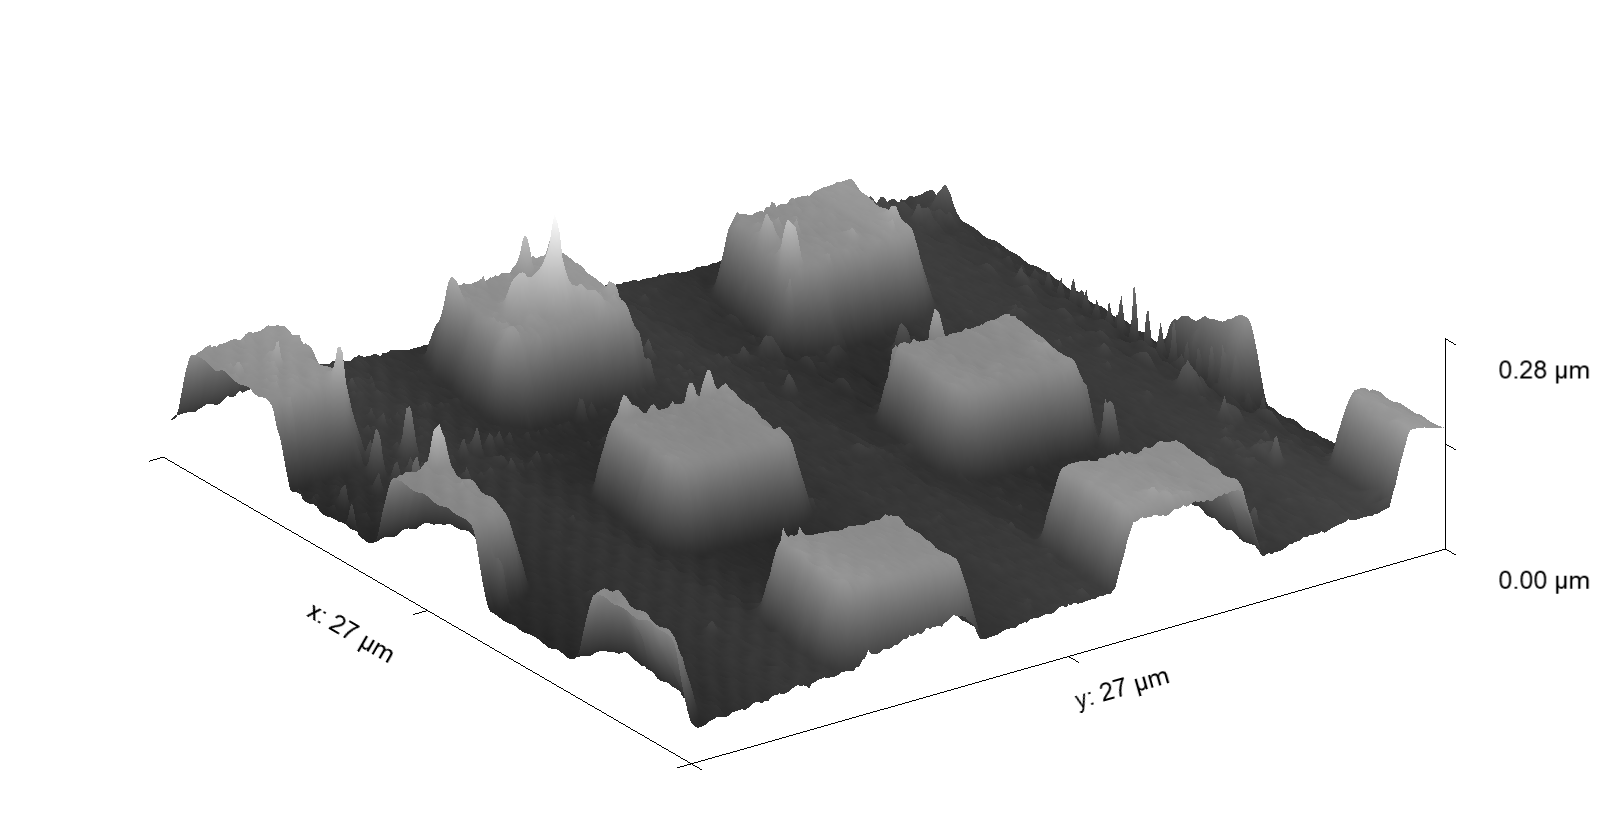
\includegraphics[width=.49\linewidth]{images/Kali/3D}}
			\subcaptionbox{Profil 1 \label{fig_kali_profil}}{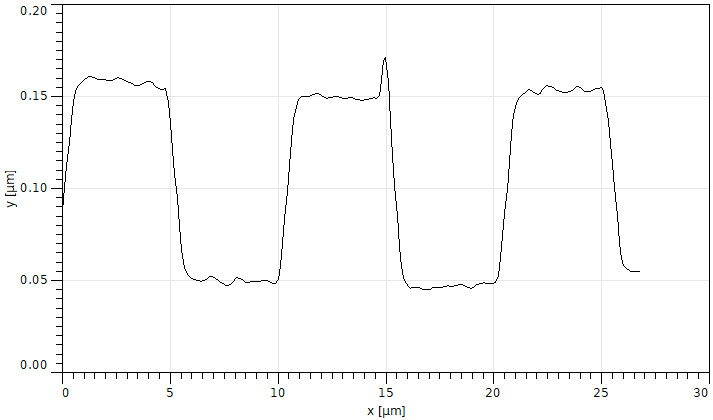
\includegraphics[width=.7\linewidth]{images/Kali/Profil}}
			\caption{Kalibrierungsprobe.}
\end{figure}

\begin{figure}[H]
			\centering
			\subcaptionbox{ \label{fig_kali_ds1}}{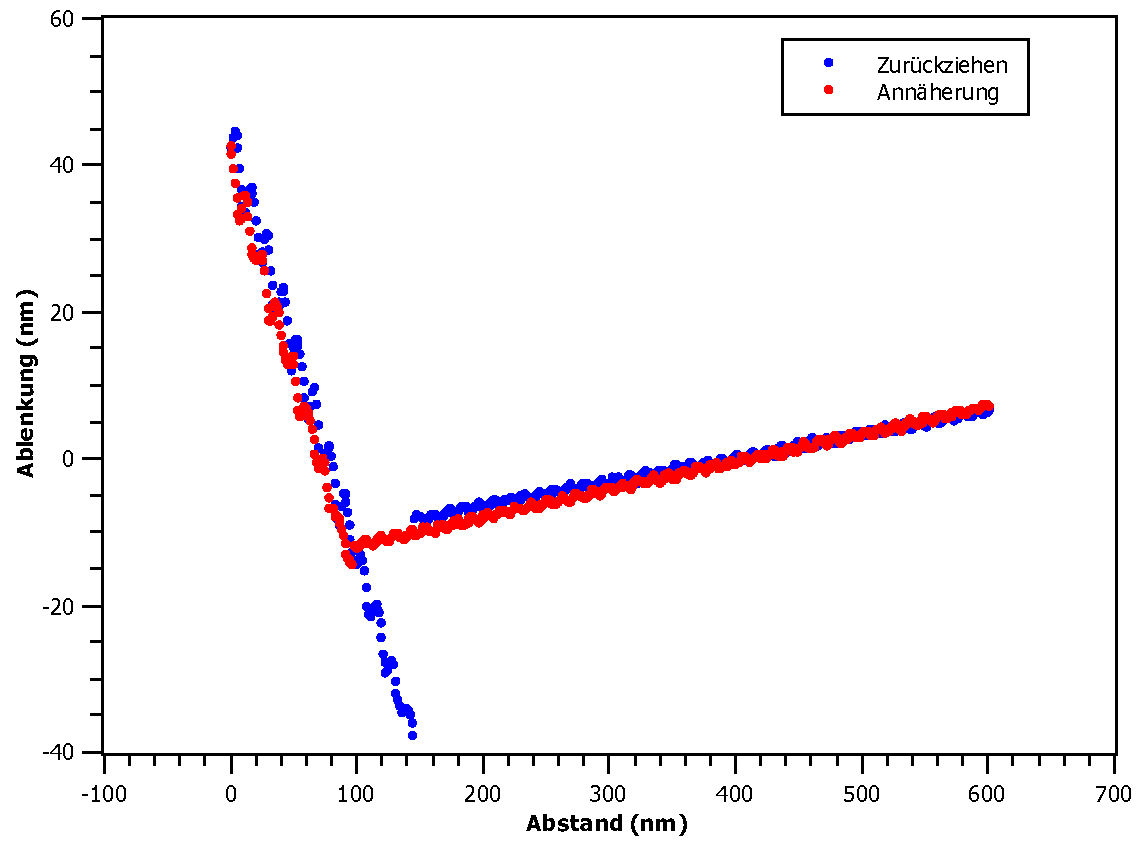
\includegraphics[width=.49\linewidth]{images/Kali/DS1}}
			\subcaptionbox{ \label{fig_kali_ds2}}{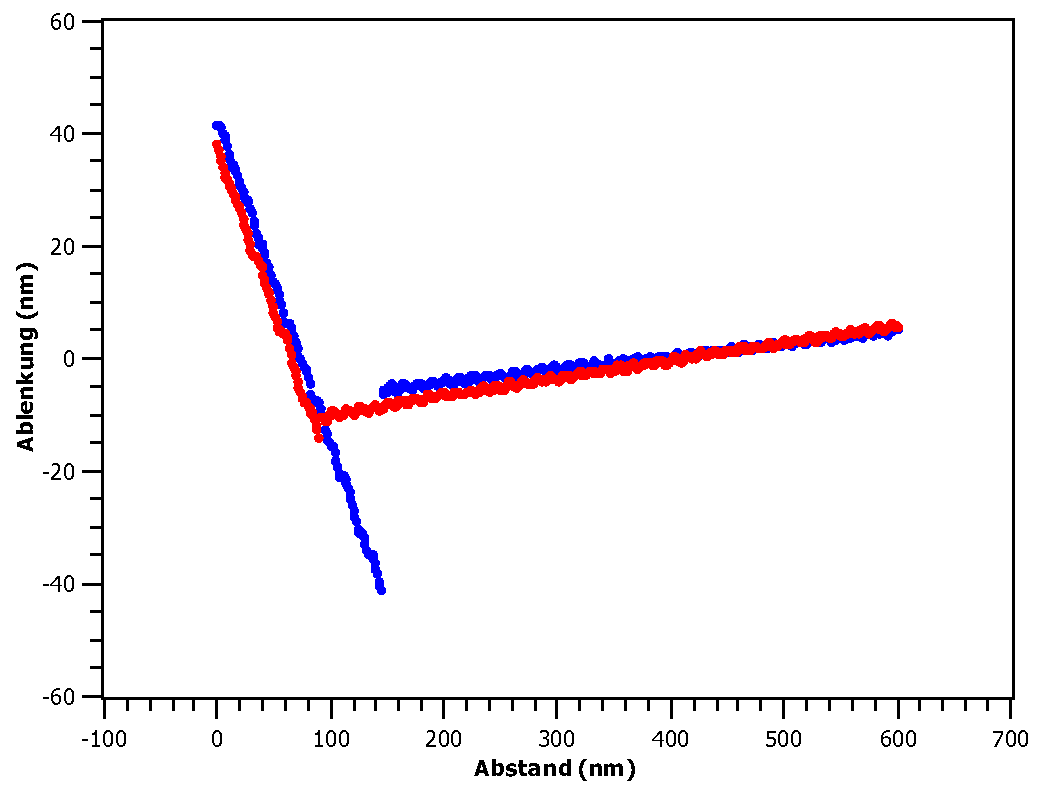
\includegraphics[width=.49\linewidth]{images/Kali/DS2}}
			\subcaptionbox{ \label{fig_kali_ds3}}{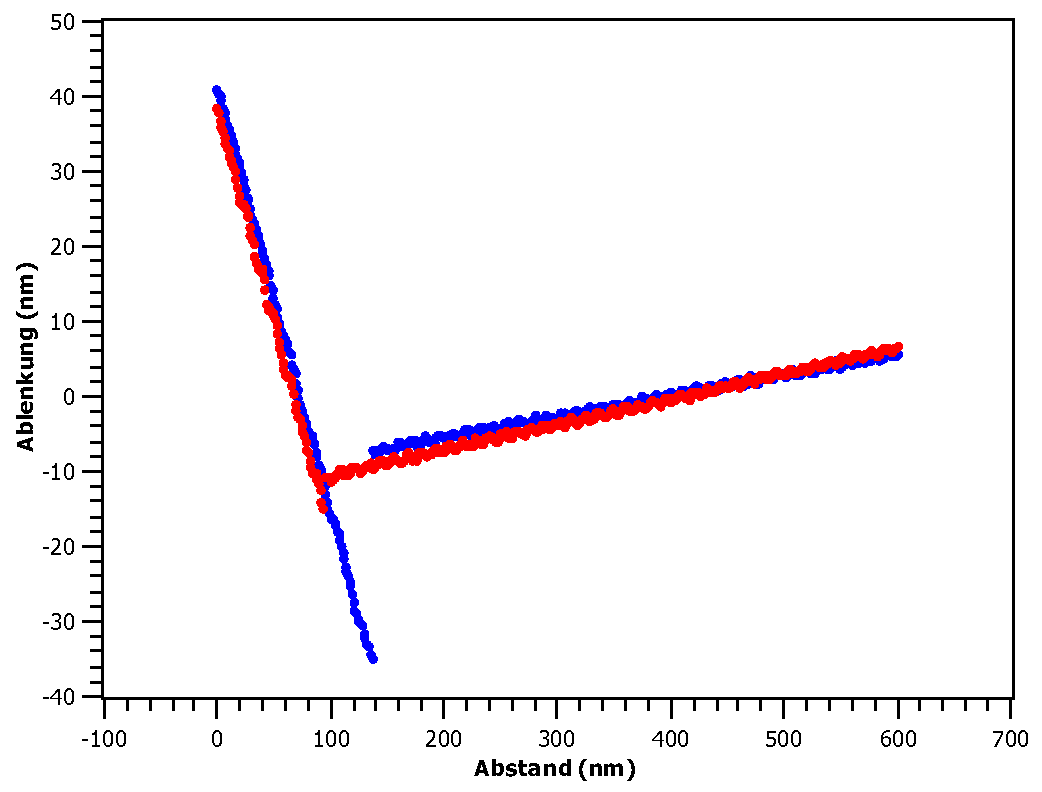
\includegraphics[width=.49\linewidth]{images/Kali/DS3}}
			\subcaptionbox{ \label{fig_kali_ds4}}{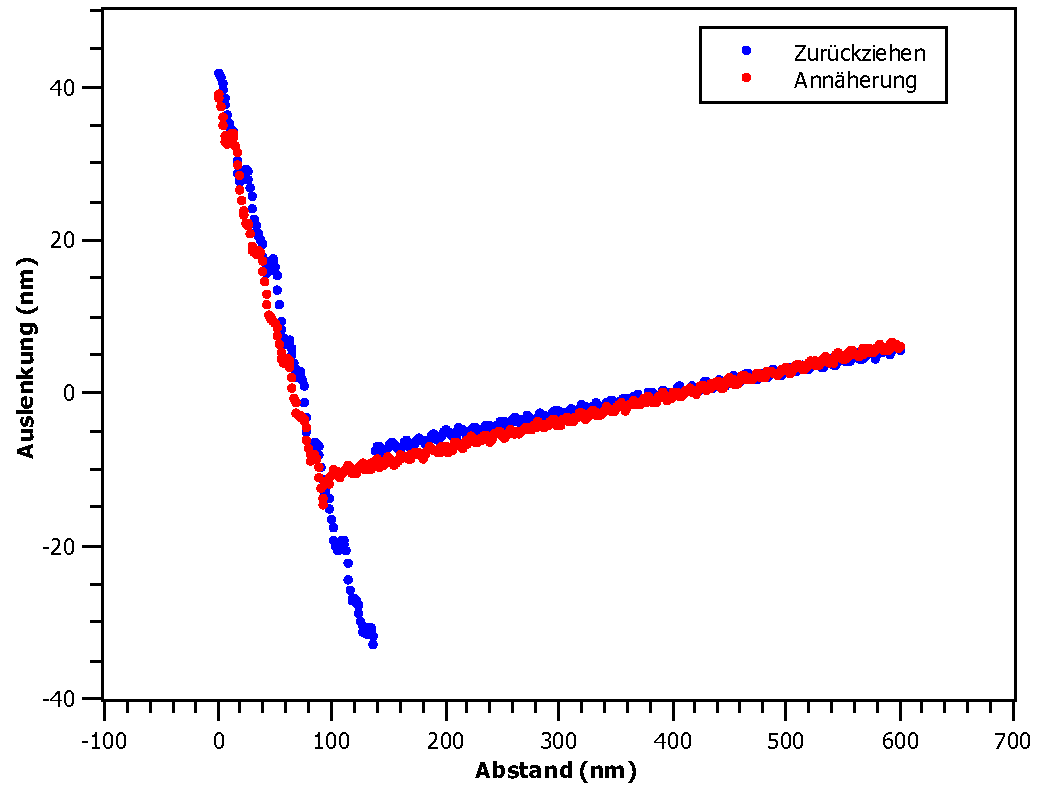
\includegraphics[width=.49\linewidth]{images/Kali/DS4}}
			\subcaptionbox{
			\label{fig_kali_ds5}}{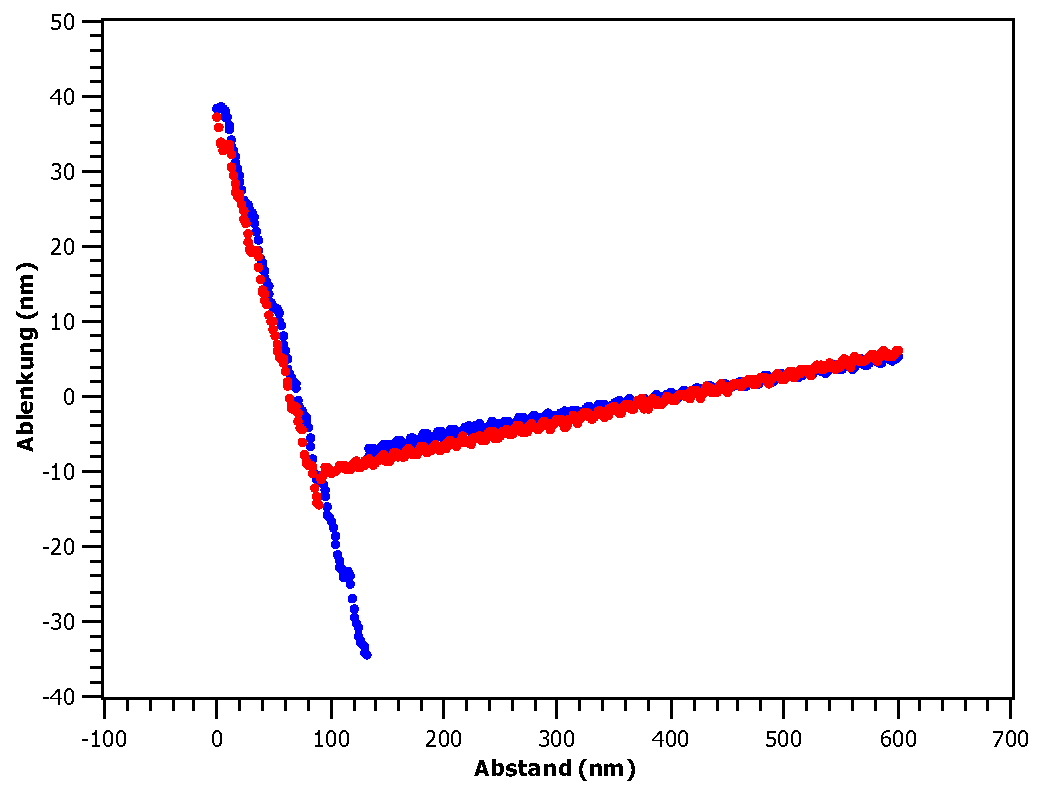
\includegraphics[width=.49\linewidth]{images/Kali/DS5}}
			\caption{Kraft-Abstands-Spektroskopie der Kalibrierungsprobe.}
\end{figure}

\begin{figure}[H]
			\subcaptionbox{Draufsicht \label{fig_dvd_top}}{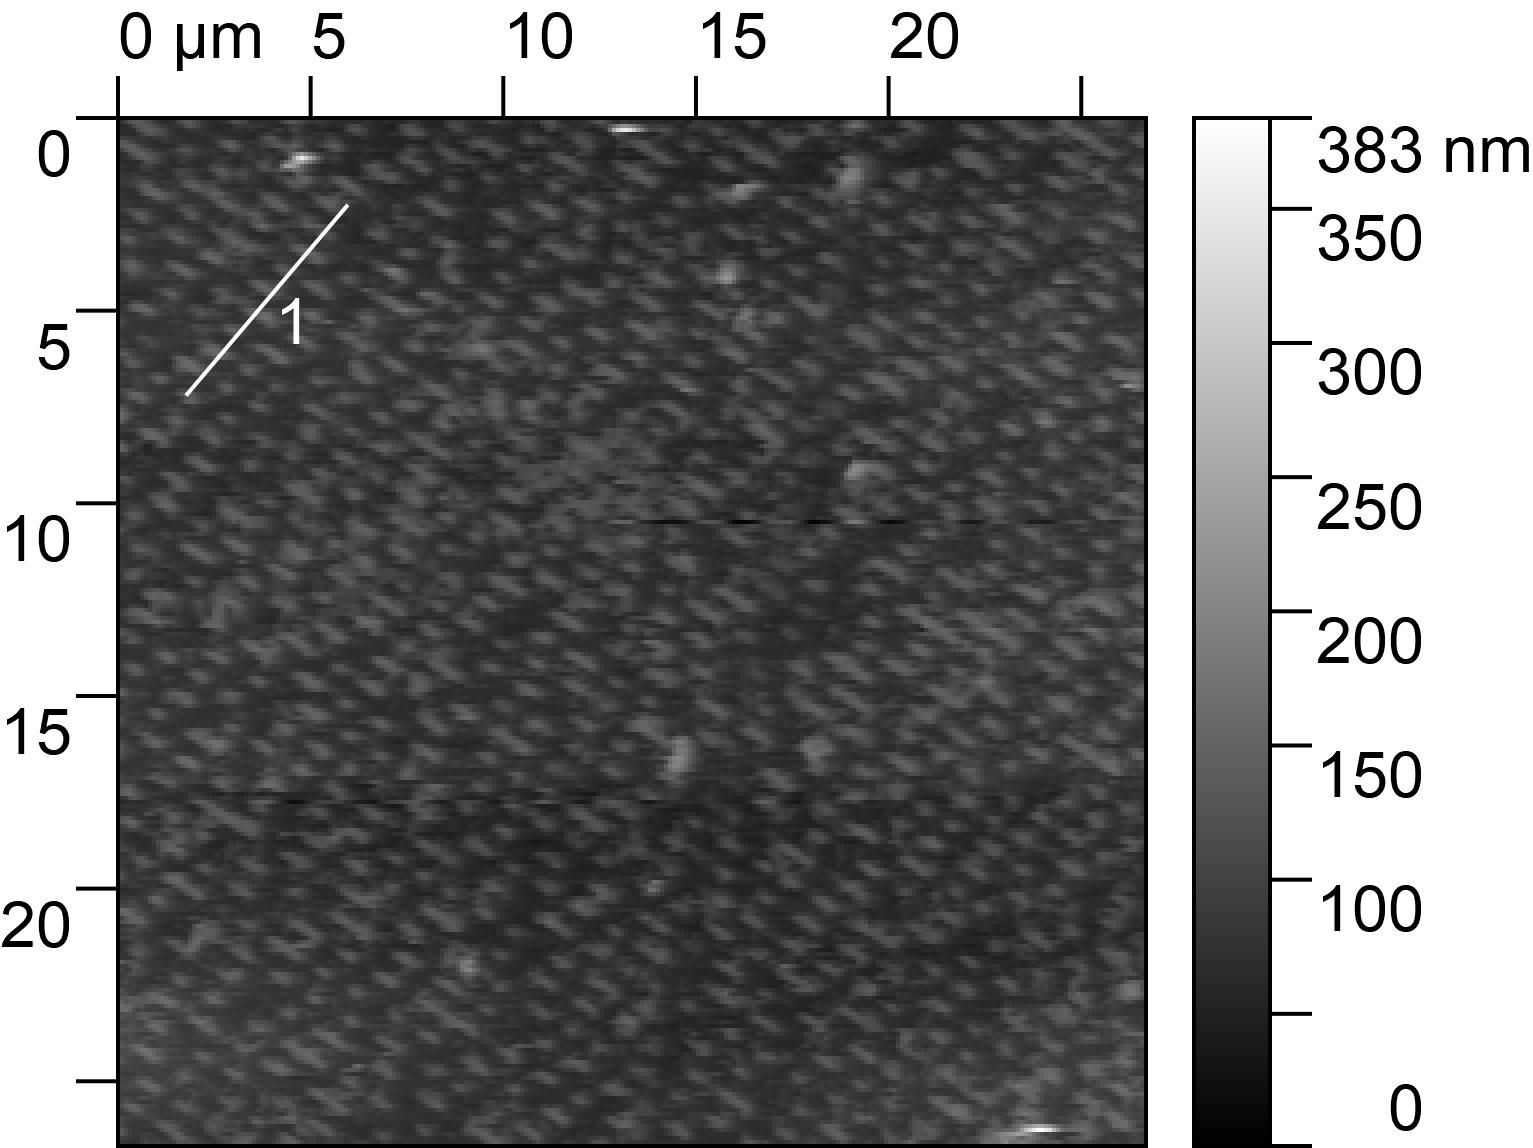
\includegraphics[width=.49\linewidth]{images/DVD/Top}}
			\subcaptionbox{3D-Sicht \label{fig_dvd_3d}}{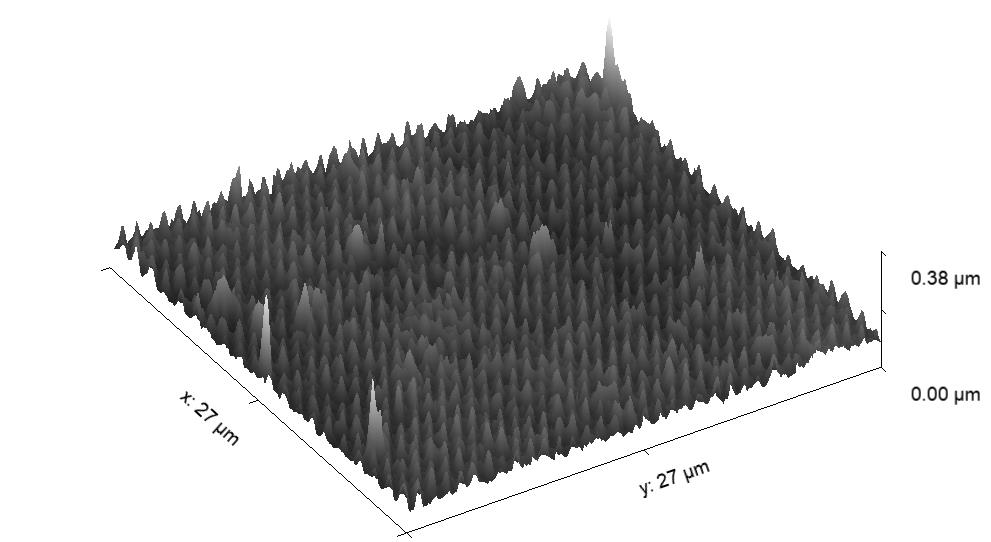
\includegraphics[width=.49\linewidth]{images/DVD/3D}}
			\subcaptionbox{Vergrößerte Draufsicht \label{fig_dvd_top_zoom}}{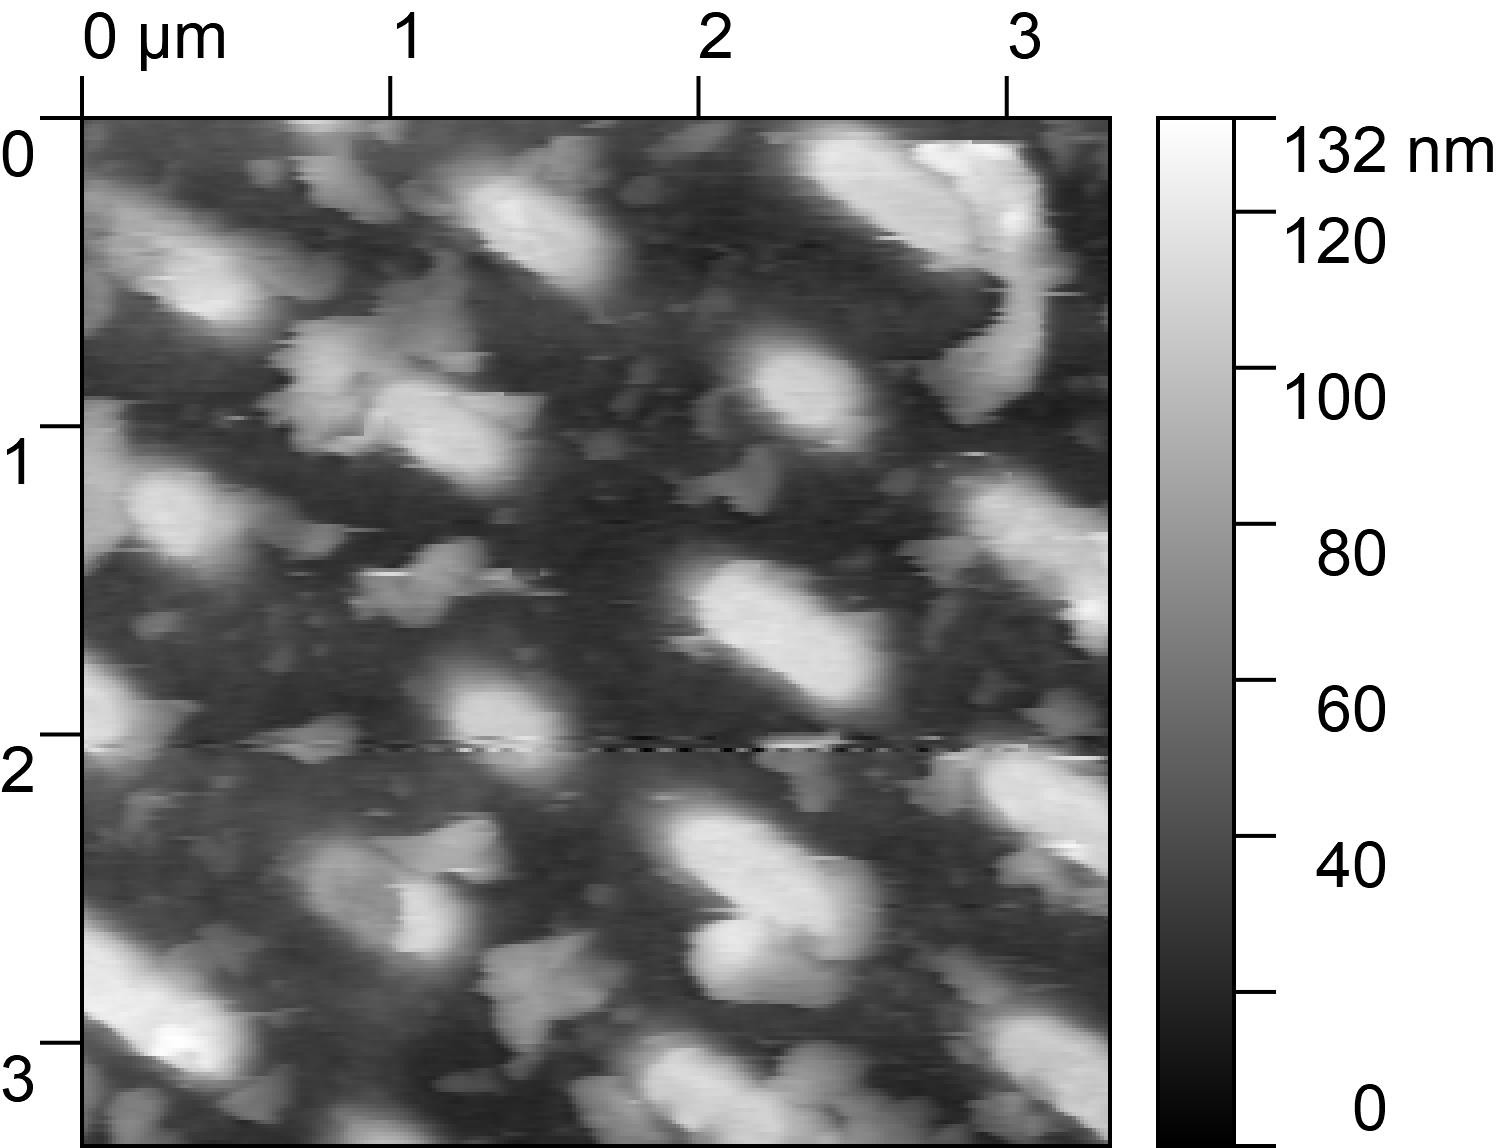
\includegraphics[width=.49\linewidth]{images/DVD/Top_zoom}}
			\subcaptionbox{Vergrößerte 3D-Sicht \label{fig_dvd_3d}}{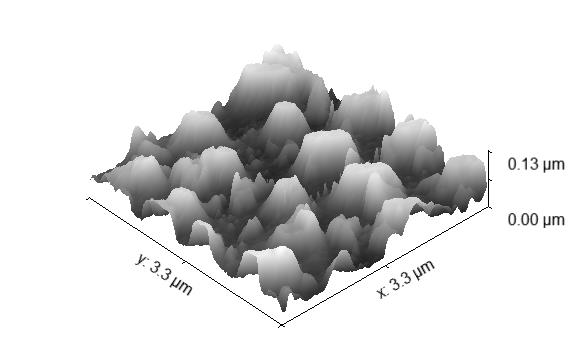
\includegraphics[width=.49\linewidth]{images/DVD/3D_zoom}}
			\subcaptionbox{Profil 1 \label{fig_dvd_profil}}{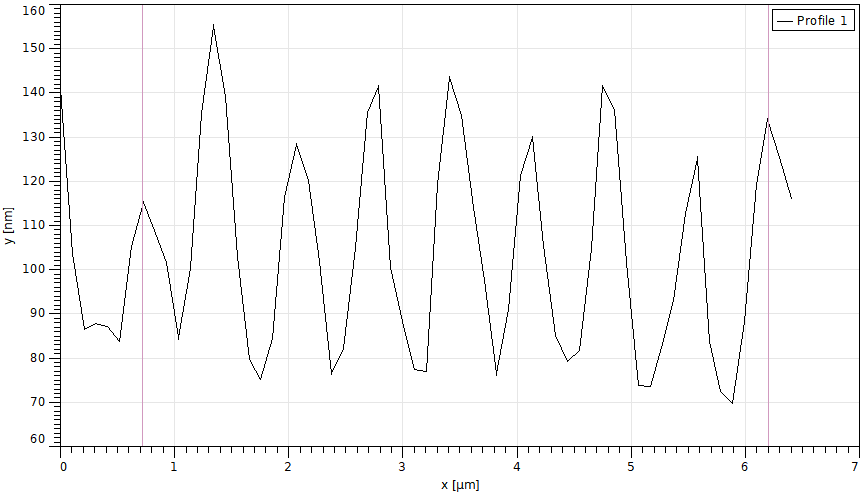
\includegraphics[width=.7\linewidth]{images/DVD/Profil}}
			\caption{Probe 1. Der Abstand gemessene Abstand in (e) beträgt \SI{5.48}{\mu m}}
\end{figure}



\end{document}
